As of right now, there is a simple statistics page that is implemented on the frontend for showing statistics for a specific course. A teacher can see pie-charts for each assignment in the course and how many students that has completed that assignment of the ones who are registered to the course.

The current implementation is using the API call to get all features for that specific course. This API call returns a lot of data that is unnecessary, and in some cases might not be correct to send to frontend. The data used for statistics has to be individually picked out from the massive response that the API call returns. In the future, it might be good to create a route from backend that returns the amount of students that has passed a specific assignment.

In the future, it might be nice to add a graph like the one in figure~\ref{fig:progovertime} for each assignment plotting when students pass a specific assignment. This feature would require the database to keep track of which dates students first pass specific assignments.
\begin{figure}[hb]
    \centering
    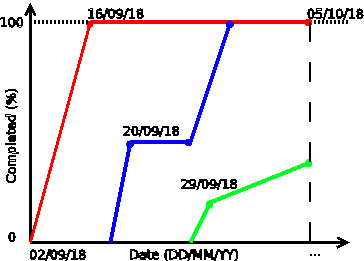
\includegraphics[width=.6\linewidth]{img_src/progress_over_time.png}
    \caption{What a time-progress graph could look like. Here, each color represents an assignment, but it could also be split into individual graphs.}\label{fig:progovertime}
\end{figure}
